\chapter{Cristais II: sólidos iônicos, covalentes e moleculares}\label{ch:b1:crystals-ionic-covalent}

O sal de cozinha, triturado, quebra-se em cubinhos; o diamante é o
material natural mais duro, e no entanto o grafite, feito dos mesmos
átomos de carbono, é mole o bastante para escrever; o gelo flutua na
água. Todos são \omterm{def:b1:crystals-metals:crystal}{cristais}, mas suas partículas se mantêm unidas de
maneiras diferentes: íons por atração eletrostática, átomos por \omterm{def:b1:lewis-resonance-vsepr:lewis}{ligações
covalentes}, moléculas pelas forças intermoleculares do
\cref{ch:b1:intermolecular-forces-solvents}. Este capítulo aplica a
geometria das células do capítulo anterior a essas três famílias de
sólidos e explica, a partir dos tamanhos dos íons, por que o cloreto de
sódio e o cloreto de césio adotam estruturas diferentes.

\begin{recall}
A \omterm{def:b1:crystals-metals:multiplicity}{multiplicidade}, o \omterm{def:b1:crystals-metals:coordination}{número de coordenação} e a \omterm{def:b1:crystals-metals:compactness}{compacidade} de uma célula,
assim como os \omterm{def:b1:crystals-metals:site}{sítios octaédricos} e tetraédricos da \omterm{def:b1:crystals-metals:lattice}{rede} \omterm{def:b1:crystals-metals:packings}{cúbica de faces
centradas}, foram definidos no \cref{ch:b1:crystals-metals}; a massa
específica de um \omterm{def:b1:crystals-metals:crystal}{cristal} é $\rho = ZM/(N_A V)$
(\cref{prop:b1:crystals-metals:density}). Os \omterm{def:b1:periodicity:radius}{raios iônicos} foram
introduzidos na \cref{def:b1:periodicity:radius}.
\end{recall}

\section{Cristais iônicos e razões de raios}

\begin{definition}[Cristal iônico]\label{def:b1:crystals-ionic-covalent:ionic-crystal}
Um \emph{cristal iônico}\index{cristal ionico@cristal iônico} é um \omterm{def:b1:crystals-metals:crystal}{cristal} de cátions e
ânions mantidos unidos por atração eletrostática. Cada íon está cercado
por íons de carga oposta; o \omterm{def:b1:crystals-metals:crystal}{cristal} é eletricamente neutro, de modo que
os números de cátions e de ânions em uma célula estão na proporção da
fórmula.
\end{definition}

\begin{proposition}[Propriedades dos cristais iônicos]\label{prop:b1:crystals-ionic-covalent:ionic-properties}
Os \omterm{def:b1:crystals-ionic-covalent:ionic-crystal}{cristais iônicos} são duros, mas quebradiços (o deslocamento de uma
camada põe frente a frente íons de mesmo sinal, e o \omterm{def:b1:crystals-metals:crystal}{cristal} se cliva),
têm altas temperaturas de fusão, não conduzem no estado sólido, mas
conduzem quando fundidos ou dissolvidos, e se dissolvem em \omterm{def:b1:intermolecular-forces-solvents:solvent-classes}{solventes
polares} de alta permissividade.
\end{proposition}
\admitted

\begin{definition}[Razão de raios]\label{def:b1:crystals-ionic-covalent:radius-ratio}
Em um \omterm{def:b1:crystals-ionic-covalent:ionic-crystal}{cristal iônico} de um cátion de raio $r_+$ e um ânion de raio
$r_-$, a \emph{razão de raios}\index{razao de raios@razão de raios} é $x = r_+/r_-$
(em geral $x < 1$, pois os cátions são menores que os ânions).
\end{definition}

\begin{proposition}[A regra da razão de raios]\label{prop:b1:crystals-ionic-covalent:rule}
No modelo das esferas rígidas, uma estrutura em que cada cátion toca $n$
ânions só é estável se os ânions não se tocarem entre si, o que exige
$x$ acima de um limite fixado pela geometria: $x \ge \sqrt3 - 1
\approx 0.732$ para 8 vizinhos (cubo), $x \ge \sqrt2 - 1 \approx 0.414$
para 6 (octaedro), $x \ge \sqrt{3/2} - 1 \approx 0.225$ para 4
(tetraedro). A estrutura adotada é a de maior coordenação permitida
por $x$.
\end{proposition}

\begin{proof}
O cátion fica na cavidade entre $n$ ânions em contato com ele. No
limite, os ânions também se tocam entre si. Cubo: os ânions estão nos
vértices de um cubo de aresta $2r_-$ e o cátion em seu centro, logo $r_+ +
r_- = \sqrt3\,r_-$. Octaedro: quatro ânions em um quadrado de
lado $2r_-$, o cátion em seu centro, $r_+ + r_- = \sqrt2\,r_-$.
Tetraedro: os ânions em vértices alternados de um cubo de aresta
$\sqrt2\,r_-$, o cátion no centro,
$r_+ + r_- = \frac{\sqrt3}{2}\sqrt2\,r_- = \sqrt{3/2}\,r_-$.
Dividindo por $r_-$, obtêm-se os limites. Abaixo do limite, o cátion
fica solto em uma cavidade grande demais para ele: os ânions se repelem
sem que a atração aumente, de modo que uma coordenação menor, com uma
cavidade menor, é preferida.
\end{proof}

\begin{omfigure}
\begin{tikzpicture}[font=\small, >={Stealth}]
  \draw[->, thick] (0,0) -- (12.4,0) node[right] {$x = r_+/r_-$};
  \foreach \x/\l in {0/0, 2.7/0.225, 4.97/0.414, 8.78/0.732, 12/1} {
    \draw (\x,0.12) -- (\x,-0.12) node[below] {\l};
  }
  \fill[omDef!15] (2.7,0.2) rectangle (4.97,1.0);
  \fill[omProp!15] (4.97,0.2) rectangle (8.78,1.0);
  \fill[omThm!15] (8.78,0.2) rectangle (12,1.0);
  \node[align=center] at (3.83,0.6) {4: ZnS};
  \node[align=center] at (6.87,0.6) {6: NaCl};
  \node[align=center] at (10.4,0.6) {8: CsCl};
  \foreach \x/\l in {3.91/\ce{ZnS}, 6.76/\ce{NaCl}, 10.08/\ce{RbCl}, 11.54/\ce{CsCl}} {
    \draw[omExo, thick] (\x,-0.55) -- (\x,-0.95);
    \node[below, omExo] at (\x,-0.95) {\l};
  }
\end{tikzpicture}

{\small A regra da \omterm{def:b1:crystals-ionic-covalent:radius-ratio}{razão de raios}: o \omterm{def:b1:crystals-metals:coordination}{número de coordenação} do cátion
permitido por $x$, e as razões medidas de quatro sais (raios de Shannon).
O cloreto de rubídio, com 0.84, deveria ser do tipo \ce{CsCl}, mas adota
o tipo \ce{NaCl}: a regra é um guia, não uma lei
(\cref{exo:b1:crystals-ionic-covalent:12}).}
% ledger: rion:Zn2+IV, rion:S2-VI, rion:Na+VI, rion:Cl-VI, rion:Rb+VI,
% rion:Cs+VIII
\end{omfigure}

\section{Quatro tipos estruturais}

\begin{definition}[Tipos estruturais]\label{def:b1:crystals-ionic-covalent:structure-type}
Os \omterm{def:b1:crystals-ionic-covalent:ionic-crystal}{cristais iônicos} são classificados em alguns tipos estruturais,
designados por um composto representativo:
\begin{itemize}
  \item \emph{tipo cloreto de césio}\index{tipo cloreto de cesio@tipo cloreto de césio}: ânions
        nos vértices de um cubo, o cátion em seu centro (8:8);
  \item \emph{tipo sal-gema}\index{tipo sal-gema} (tipo cloreto de
        sódio): ânions em uma \omterm{def:b1:crystals-metals:lattice}{rede} CFC, cátions em todos os seus \omterm{def:b1:crystals-metals:site}{sítios
        octaédricos} (6:6);
  \item \emph{tipo blenda}\index{tipo blenda} (blenda de zinco): ânions
        em uma \omterm{def:b1:crystals-metals:lattice}{rede} CFC, cátions na metade de seus \omterm{def:b1:crystals-metals:site}{sítios tetraédricos},
        um em cada dois, alternadamente (4:4);
  \item \emph{tipo fluorita}\index{tipo fluorita}: cátions em uma \omterm{def:b1:crystals-metals:lattice}{rede}
        CFC, ânions em todos os seus \omterm{def:b1:crystals-metals:site}{sítios tetraédricos} (8:4), fórmula
        \ce{MX2}; no \emph{tipo antifluorita}\index{tipo antifluorita},
        os papéis se invertem (\ce{Li2O}, 4:8).
\end{itemize}
O par de números dá a coordenação do cátion e a do ânion.
\end{definition}

\begin{omfigure}
\tdplotsetmaincoords{60}{100}
\begin{tikzpicture}[tdplot_main_coords, font=\small]
  \pic {omcubeo={3}};
    \node[aX={green!55!black}{6.5mm}] at (0,0,0) {};
  \node[aX={violet!70}{3.8mm}] at (0,1.5,0) {};
  \node[aX={green!55!black}{6.5mm}] at (0,3,0) {};
  \node[aX={violet!70}{3.8mm}] at (0,0,1.5) {};
  \node[aX={green!55!black}{6.5mm}] at (0,1.5,1.5) {};
  \node[aX={violet!70}{3.8mm}] at (0,3,1.5) {};
  \node[aX={violet!70}{3.8mm}] at (1.5,0,0) {};
  \node[aX={green!55!black}{6.5mm}] at (0,0,3) {};
  \node[aX={green!55!black}{6.5mm}] at (1.5,1.5,0) {};
  \node[aX={violet!70}{3.8mm}] at (0,1.5,3) {};
  \node[aX={violet!70}{3.8mm}] at (1.5,3,0) {};
  \node[aX={green!55!black}{6.5mm}] at (0,3,3) {};
  \node[aX={green!55!black}{6.5mm}] at (1.5,0,1.5) {};
  \node[aX={violet!70}{3.8mm}] at (1.5,1.5,1.5) {};
  \node[aX={green!55!black}{6.5mm}] at (1.5,3,1.5) {};
  \node[aX={green!55!black}{6.5mm}] at (3,0,0) {};
  \node[aX={violet!70}{3.8mm}] at (1.5,0,3) {};
  \node[aX={violet!70}{3.8mm}] at (3,1.5,0) {};
  \node[aX={green!55!black}{6.5mm}] at (1.5,1.5,3) {};
  \node[aX={green!55!black}{6.5mm}] at (3,3,0) {};
  \node[aX={violet!70}{3.8mm}] at (1.5,3,3) {};
  \node[aX={violet!70}{3.8mm}] at (3,0,1.5) {};
  \node[aX={green!55!black}{6.5mm}] at (3,1.5,1.5) {};
  \node[aX={violet!70}{3.8mm}] at (3,3,1.5) {};
  \node[aX={green!55!black}{6.5mm}] at (3,0,3) {};
  \node[aX={violet!70}{3.8mm}] at (3,1.5,3) {};
  \node[aX={green!55!black}{6.5mm}] at (3,3,3) {};
  \node at (1.5,1.5,-1.75) {\ce{NaCl} (sal-gema)};
\end{tikzpicture}
\hspace{1cm}
\begin{tikzpicture}[tdplot_main_coords, font=\small]
  \pic {omcubeo={3}};
    \node[aX={green!55!black}{6.5mm}] at (0,0,0) {};
  \node[aX={green!55!black}{6.5mm}] at (0,3,0) {};
  \node[aX={green!55!black}{6.5mm}] at (0,0,3) {};
  \node[aX={green!55!black}{6.5mm}] at (0,3,3) {};
  \node[aX={blue!60}{7mm}] at (1.5,1.5,1.5) {};
  \node[aX={green!55!black}{6.5mm}] at (3,0,0) {};
  \node[aX={green!55!black}{6.5mm}] at (3,3,0) {};
  \node[aX={green!55!black}{6.5mm}] at (3,0,3) {};
  \node[aX={green!55!black}{6.5mm}] at (3,3,3) {};
  \node at (1.5,1.5,-1.75) {\ce{CsCl}};
\end{tikzpicture}

{\small À esquerda: a célula do sal-gema, \ce{Cl-} (verde) em uma \omterm{def:b1:crystals-metals:lattice}{rede}
CFC, \ce{Na+} (violeta) em todos os \omterm{def:b1:crystals-metals:site}{sítios octaédricos}. À direita: a
célula do cloreto de césio, \ce{Cl-} nos vértices, \ce{Cs+} (azul) no
centro. Íons desenhados menores que em contato.}
\end{omfigure}

\begin{proposition}[Tipos sal-gema e cloreto de césio]\label{prop:b1:crystals-ionic-covalent:nacl-cscl}
No \omterm{def:b1:crystals-ionic-covalent:structure-type}{tipo sal-gema}, há $Z = 4$ unidades de fórmula por célula, os íons se
tocam ao longo de uma aresta, $a = 2(r_+ + r_-)$, e a estrutura exige
$\sqrt2 - 1
\le x$. No \omterm{def:b1:crystals-ionic-covalent:structure-type}{tipo cloreto de césio}, $Z = 1$, os íons se tocam
ao longo da diagonal principal, $a\sqrt3 = 2(r_+ + r_-)$, e a estrutura
exige
$x \ge \sqrt3 - 1$.
\end{proposition}

\begin{proof}
Sal-gema: os ânions da \omterm{def:b1:crystals-metals:lattice}{rede} CFC contam $4$; os cátions nos 4 \omterm{def:b1:crystals-metals:site}{sítios
octaédricos}, $1 + 12 \times \frac14 = 4$. Ao longo de uma aresta,
ânion, cátion e ânion se sucedem em contato. Os ânions não se
interpenetram se a diagonal de face, que contém três ânions dos quais
dois no máximo se tocam, satisfaz $a\sqrt2 \ge 4r_-$, ou seja,
$2(r_+ + r_-)\sqrt2 \ge
4r_-$, ou $x \ge \sqrt2 - 1$. Cloreto de césio: $8 \times \frac18 = 1$
ânion e 1 cátion; na diagonal principal, ânion, cátion e ânion em
contato; os ânions não se interpenetram ao longo de uma aresta se
$a \ge 2r_-$, ou seja,
$2(r_+ + r_-)/\sqrt3 \ge 2r_-$, ou $x \ge \sqrt3 - 1$.
\end{proof}

\begin{example}[Cloreto de sódio e cloreto de césio]\label{ex:b1:crystals-ionic-covalent:nacl}
O cloreto de sódio tem $a = \qty{564.1}{pm}$: $r_+ + r_- = a/2 =
\qty{282.0}{pm}$, contra $102 + 181 = \qty{283}{pm}$ pelos raios de
Shannon; $x = 102/181 = 0.56$, na faixa octaédrica. Sua massa específica
é $\rho = 4 \times 58.44/(6.022 \times 10^{23} \times (5.641 \times
10^{-8})^3) = \qty{2.16}{g/cm^3}$; medida: \qty{2.17}{g/cm^3}. O cloreto
de césio tem $a = \qty{412.3}{pm}$: $r_+ + r_- = a\sqrt3/2 =
\qty{357.1}{pm}$, e $x = 174/181 = 0.96$, na faixa cúbica.
% ledger: lat:NaCl, rion:Na+VI, rion:Cl-VI, rho:NaCl, lat:CsCl,
% rion:Cs+VIII
\end{example}

\begin{omfigure}
\begin{minipage}[b]{0.31\linewidth}\centering
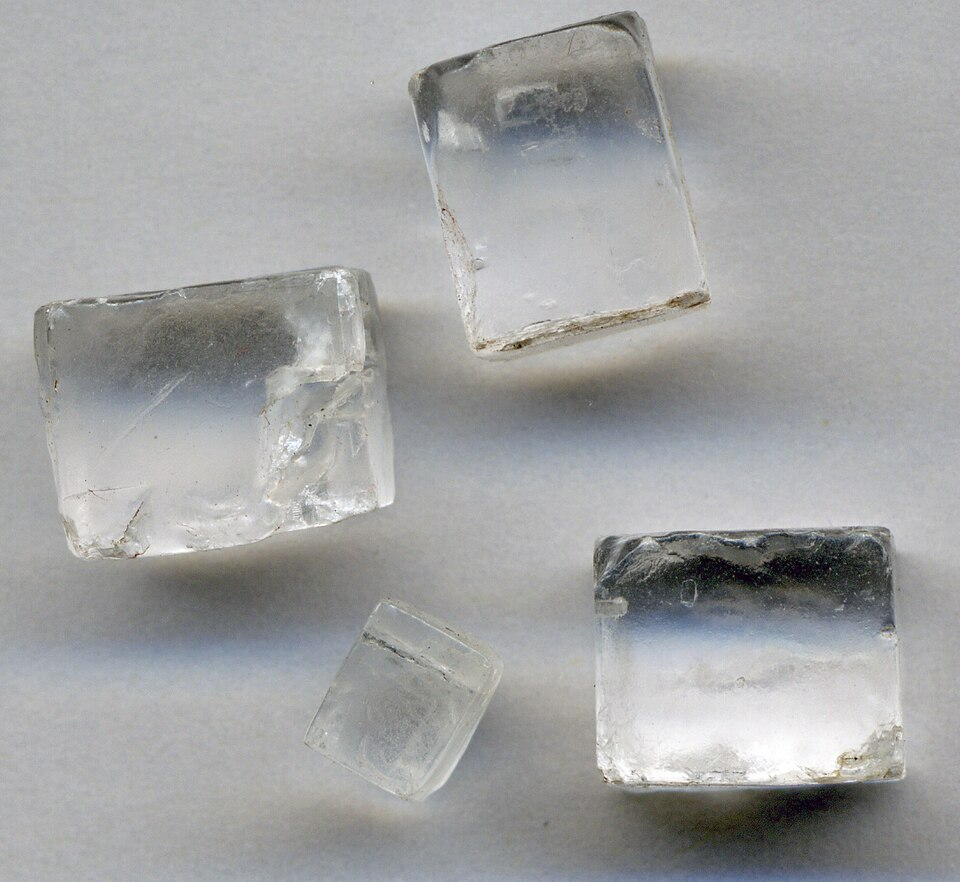
\includegraphics[width=\linewidth]{images/book2/halite.jpg}

{\small \omterm{def:b1:crystals-metals:crystal}{Cristais} de halita (sal-gema). Foto: James St. John, CC BY 2.0.}
\end{minipage}\hfill
\begin{minipage}[b]{0.31\linewidth}\centering
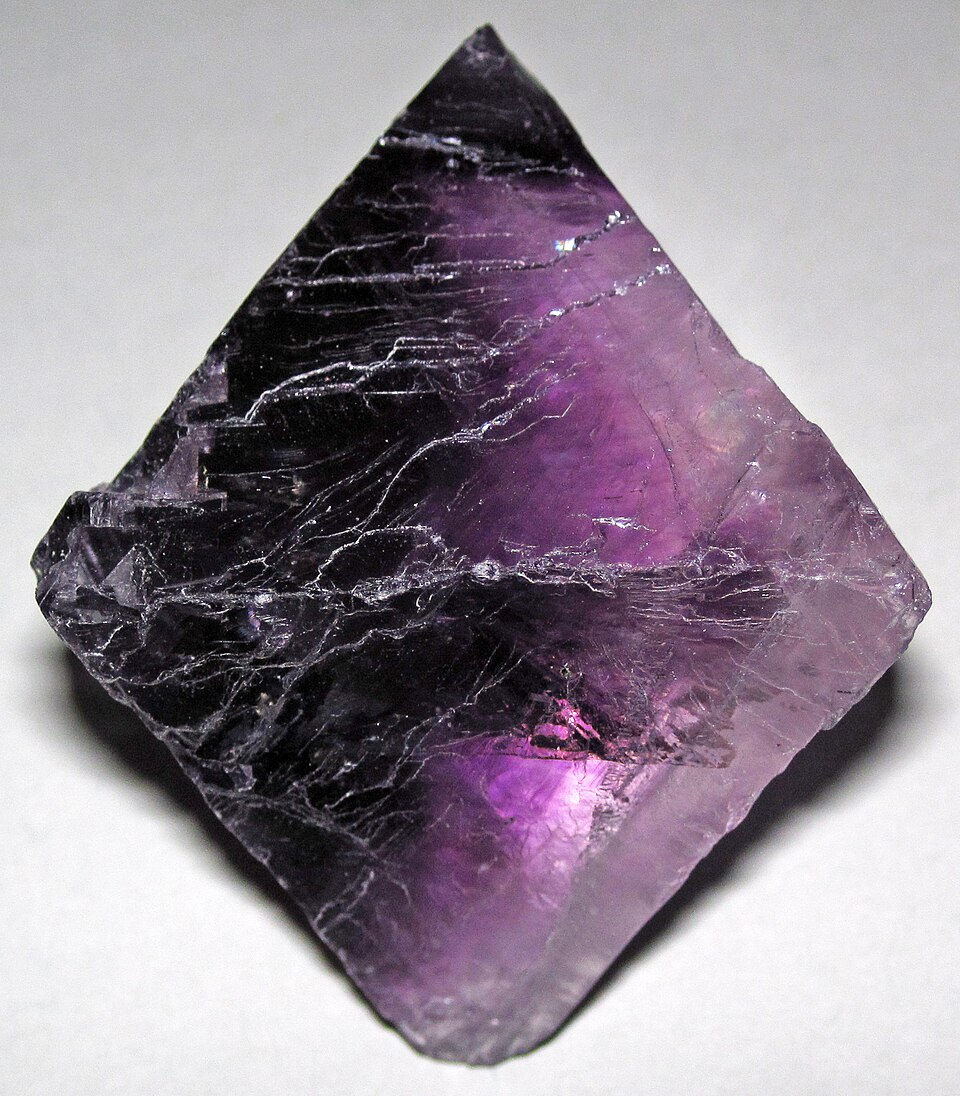
\includegraphics[width=0.85\linewidth]{images/book2/fluorite.jpg}

{\small Fluorita, \ce{CaF2}. Foto: James St. John, CC BY 2.0.}
\end{minipage}\hfill
\begin{minipage}[b]{0.31\linewidth}\centering
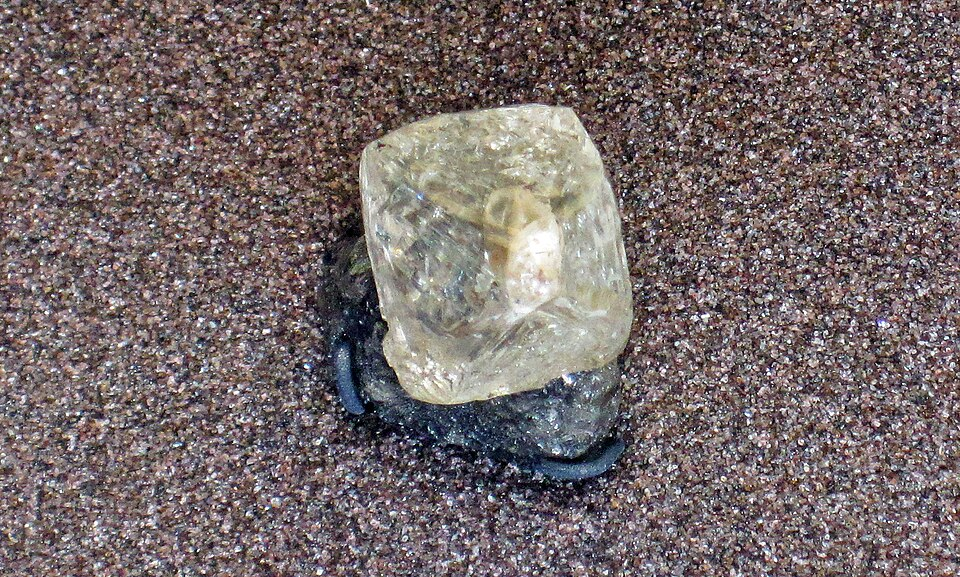
\includegraphics[width=\linewidth]{images/book2/diamond.jpg}

{\small Um octaedro de diamante bruto. Foto: James St. John, CC BY 2.0.}
\end{minipage}
\end{omfigure}

\begin{proposition}[Tipos blenda e fluorita]\label{prop:b1:crystals-ionic-covalent:zns-caf2}
No \omterm{def:b1:crystals-ionic-covalent:structure-type}{tipo blenda}, $Z = 4$, cada íon está cercado por quatro íons do outro
tipo nos vértices de um tetraedro, e os íons se tocam ao longo de um
quarto da diagonal principal: $a\sqrt3/4 = r_+ + r_-$. No \omterm{def:b1:crystals-ionic-covalent:structure-type}{tipo fluorita},
$Z = 4$ unidades \ce{CaF2}, cada cátion tem 8 ânions vizinhos (um cubo),
cada ânion 4 cátions vizinhos (um tetraedro), e de novo $a\sqrt3/4 =
r_+ + r_-$.
\end{proposition}

\begin{proof}
Blenda: 4 ânions na \omterm{def:b1:crystals-metals:lattice}{rede} CFC e 4 cátions na metade dos 8 \omterm{def:b1:crystals-metals:site}{sítios
tetraédricos}. Um \omterm{def:b1:crystals-metals:site}{sítio tetraédrico} em $(\frac a4,\frac a4,\frac a4)$
fica a $\frac{a\sqrt3}{4}$ de seus quatro ânions. Fluorita: 4 cátions e
8 ânions em todos os \omterm{def:b1:crystals-metals:site}{sítios tetraédricos}, razão $1:2$. Os 8 ânions
internos à célula formam um cubo de aresta $a/2$, e os cubinhos de
ânions contêm, um sim, um não, um cátion em seu centro; um ânion tem
seus 4 cátions vizinhos a $\frac{a\sqrt3}{4}$.
\end{proof}

\begin{omfigure}
\tdplotsetmaincoords{60}{100}
\begin{tikzpicture}[tdplot_main_coords, font=\small]
  \pic {omcubeo={3}};
  \begin{scope}[on background layer]
    \draw[black!45, line width=1.2pt] (0.75,0.75,2.25) -- (0,0,3) (0.75,0.75,2.25) -- (0,1.5,1.5) (0.75,0.75,2.25) -- (1.5,0,1.5) (0.75,0.75,2.25) -- (1.5,1.5,3) (0.75,2.25,0.75) -- (0,1.5,1.5) (0.75,2.25,0.75) -- (0,3,0) (0.75,2.25,0.75) -- (1.5,1.5,0) (0.75,2.25,0.75) -- (1.5,3,1.5) (2.25,0.75,0.75) -- (1.5,0,1.5) (2.25,0.75,0.75) -- (1.5,1.5,0) (2.25,0.75,0.75) -- (3,0,0) (2.25,0.75,0.75) -- (3,1.5,1.5) (2.25,2.25,2.25) -- (1.5,1.5,3) (2.25,2.25,2.25) -- (1.5,3,1.5) (2.25,2.25,2.25) -- (3,1.5,1.5) (2.25,2.25,2.25) -- (3,3,3);
  \end{scope}
    \node[aX={yellow!75!orange}{6mm}] at (0,0,0) {};
  \node[aX={yellow!75!orange}{6mm}] at (0,3,0) {};
  \node[aX={yellow!75!orange}{6mm}] at (0,1.5,1.5) {};
  \node[aX={gray!60}{3.6mm}] at (0.75,2.25,0.75) {};
  \node[aX={yellow!75!orange}{6mm}] at (0,0,3) {};
  \node[aX={yellow!75!orange}{6mm}] at (1.5,1.5,0) {};
  \node[aX={gray!60}{3.6mm}] at (0.75,0.75,2.25) {};
  \node[aX={yellow!75!orange}{6mm}] at (0,3,3) {};
  \node[aX={yellow!75!orange}{6mm}] at (1.5,0,1.5) {};
  \node[aX={gray!60}{3.6mm}] at (2.25,0.75,0.75) {};
  \node[aX={yellow!75!orange}{6mm}] at (1.5,3,1.5) {};
  \node[aX={yellow!75!orange}{6mm}] at (3,0,0) {};
  \node[aX={yellow!75!orange}{6mm}] at (1.5,1.5,3) {};
  \node[aX={yellow!75!orange}{6mm}] at (3,3,0) {};
  \node[aX={gray!60}{3.6mm}] at (2.25,2.25,2.25) {};
  \node[aX={yellow!75!orange}{6mm}] at (3,1.5,1.5) {};
  \node[aX={yellow!75!orange}{6mm}] at (3,0,3) {};
  \node[aX={yellow!75!orange}{6mm}] at (3,3,3) {};
  \node at (1.5,1.5,-1.75) {\ce{ZnS} (blenda)};
\end{tikzpicture}
\hspace{1cm}
\begin{tikzpicture}[tdplot_main_coords, font=\small]
  \pic {omcubeo={3}};
    \node[aX={green!35!gray}{4.4mm}] at (0,0,0) {};
  \node[aX={green!35!gray}{4.4mm}] at (0,3,0) {};
  \node[aX={green!35!gray}{4.4mm}] at (0,1.5,1.5) {};
  \node[aX={green!45!yellow}{5.0mm}] at (0.75,0.75,0.75) {};
  \node[aX={green!45!yellow}{5.0mm}] at (0.75,2.25,0.75) {};
  \node[aX={green!35!gray}{4.4mm}] at (0,0,3) {};
  \node[aX={green!35!gray}{4.4mm}] at (1.5,1.5,0) {};
  \node[aX={green!45!yellow}{5.0mm}] at (0.75,0.75,2.25) {};
  \node[aX={green!35!gray}{4.4mm}] at (0,3,3) {};
  \node[aX={green!35!gray}{4.4mm}] at (1.5,0,1.5) {};
  \node[aX={green!45!yellow}{5.0mm}] at (0.75,2.25,2.25) {};
  \node[aX={green!45!yellow}{5.0mm}] at (2.25,0.75,0.75) {};
  \node[aX={green!35!gray}{4.4mm}] at (1.5,3,1.5) {};
  \node[aX={green!35!gray}{4.4mm}] at (3,0,0) {};
  \node[aX={green!45!yellow}{5.0mm}] at (2.25,2.25,0.75) {};
  \node[aX={green!35!gray}{4.4mm}] at (1.5,1.5,3) {};
  \node[aX={green!35!gray}{4.4mm}] at (3,3,0) {};
  \node[aX={green!45!yellow}{5.0mm}] at (2.25,0.75,2.25) {};
  \node[aX={green!45!yellow}{5.0mm}] at (2.25,2.25,2.25) {};
  \node[aX={green!35!gray}{4.4mm}] at (3,1.5,1.5) {};
  \node[aX={green!35!gray}{4.4mm}] at (3,0,3) {};
  \node[aX={green!35!gray}{4.4mm}] at (3,3,3) {};
  \node at (1.5,1.5,-1.75) {\ce{CaF2} (fluorita)};
\end{tikzpicture}

{\small À esquerda: a blenda, \ce{S^{2-}} (amarelo) em uma \omterm{def:b1:crystals-metals:lattice}{rede} CFC e
\ce{Zn^{2+}} (cinza) em \omterm{def:b1:crystals-metals:site}{sítios tetraédricos} alternados, cada um ligado a
seus quatro vizinhos. À direita: a fluorita, \ce{Ca^{2+}} (verde-acinzentado)
em uma \omterm{def:b1:crystals-metals:lattice}{rede} CFC e \ce{F-} (verde-claro) em todos os oito \omterm{def:b1:crystals-metals:site}{sítios
tetraédricos}.}
\end{omfigure}

\begin{example}[Blenda e fluorita]\label{ex:b1:crystals-ionic-covalent:zns}
A blenda tem $a = \qty{540.9}{pm}$: $r_+ + r_- = a\sqrt3/4 =
\qty{234.2}{pm}$ (Shannon: $60 + 184 = \qty{244}{pm}$, pois o raio do
sulfeto só é tabelado para seis vizinhos), e $x = 60/184 = 0.33$, na
faixa tetraédrica. A fluorita tem $a = \qty{546.3}{pm}$: $r_+ + r_- =
\qty{236.6}{pm}$ (Shannon: $112 + 131 = \qty{243}{pm}$), e $x = 0.85$: o
cátion fica em um cubo de 8 ânions, como a regra exige.
% ledger: lat:ZnS, rion:Zn2+IV, rion:S2-VI, lat:CaF2, rion:Ca2+VIII,
% rion:F-IV
\end{example}

\begin{method}[Prever uma estrutura]\label{met:b1:crystals-ionic-covalent:predict}
Para prever a estrutura de um composto iônico \ce{MX} ou \ce{MX2}:
\begin{enumerate}
  \item calcule $x = r_+/r_-$ a partir de raios tabelados (para a
        coordenação esperada);
  \item leia a coordenação do cátion na regra da \omterm{def:b1:crystals-ionic-covalent:radius-ratio}{razão de raios};
  \item escolha o tipo que tem essa coordenação e a fórmula correta:
        \ce{MX} com 8: \ce{CsCl}; com 6: \ce{NaCl}; com 4: blenda;
        \ce{MX2} com 8: fluorita;
  \item confira com o \omterm{def:b1:crystals-metals:lattice}{parâmetro de rede} medido; lembre que íons
        polarizáveis (\ce{S^{2-}}, \ce{I-}) e cátions pequenos e
        carregados dão ligações parcialmente covalentes, para as quais
        a regra falha.
\end{enumerate}
\end{method}

\section{Cristais covalentes}

\begin{definition}[Cristal covalente]\label{def:b1:crystals-ionic-covalent:covalent-crystal}
Um \emph{cristal covalente}\index{cristal covalente} (ou sólido
reticular) é um \omterm{def:b1:crystals-metals:crystal}{cristal} em que todos os átomos estão ligados por
\omterm{def:b1:lewis-resonance-vsepr:lewis}{ligações covalentes} em uma única molécula gigante: diamante, silício,
quartzo \ce{SiO2}. Em um \omterm{def:b1:crystals-metals:crystal}{cristal} covalente lamelar como o grafite, a
rede covalente só se estende em planos, que se mantêm unidos uns aos
outros por \omterm{def:b1:intermolecular-forces-solvents:vdw}{interações de van der Waals}.
\end{definition}

\begin{proposition}[A estrutura do diamante]\label{prop:b1:crystals-ionic-covalent:diamond}
No diamante, os átomos de carbono ocupam a \omterm{def:b1:crystals-metals:lattice}{rede} CFC e a metade de seus
\omterm{def:b1:crystals-metals:site}{sítios tetraédricos}, como os dois tipos de íons da blenda: $Z = 8$, cada
carbono ligado a outros quatro nos vértices de um tetraedro, à
distância $a\sqrt3/4$. Para esferas em contato, a \omterm{def:b1:crystals-metals:compactness}{compacidade} é
\[
  C = \frac{\pi\sqrt3}{16} \approx 0.34 .
\]
\end{proposition}

\begin{proof}
$Z = 4 + 4 = 8$. Os átomos vizinhos se tocam: $2R = a\sqrt3/4$, logo $a =
8R/\sqrt3$ e $C = 8 \cdot \frac43\pi R^3/a^3 = \frac{32}{3}\pi R^3 \cdot
\frac{3\sqrt3}{512 R^3} = \frac{\pi\sqrt3}{16}$.
\end{proof}

\begin{omfigure}
\tdplotsetmaincoords{60}{100}
\begin{tikzpicture}[tdplot_main_coords, font=\small]
  \pic {omcubeo={3}};
  \begin{scope}[on background layer]
    \draw[black!55, line width=1.4pt] (0.75,0.75,2.25) -- (0,0,3) (0.75,0.75,2.25) -- (0,1.5,1.5) (0.75,0.75,2.25) -- (1.5,0,1.5) (0.75,0.75,2.25) -- (1.5,1.5,3) (0.75,2.25,0.75) -- (0,1.5,1.5) (0.75,2.25,0.75) -- (0,3,0) (0.75,2.25,0.75) -- (1.5,1.5,0) (0.75,2.25,0.75) -- (1.5,3,1.5) (2.25,0.75,0.75) -- (1.5,0,1.5) (2.25,0.75,0.75) -- (1.5,1.5,0) (2.25,0.75,0.75) -- (3,0,0) (2.25,0.75,0.75) -- (3,1.5,1.5) (2.25,2.25,2.25) -- (1.5,1.5,3) (2.25,2.25,2.25) -- (1.5,3,1.5) (2.25,2.25,2.25) -- (3,1.5,1.5) (2.25,2.25,2.25) -- (3,3,3);
  \end{scope}
  \node[aX={black!65}{3.6mm}] at (0,0,0) {};
  \node[aX={black!65}{3.6mm}] at (0,3,0) {};
  \node[aX={black!65}{3.6mm}] at (0,1.5,1.5) {};
  \node[aX={black!65}{3.6mm}] at (0.75,2.25,0.75) {};
  \node[aX={black!65}{3.6mm}] at (0,0,3) {};
  \node[aX={black!65}{3.6mm}] at (1.5,1.5,0) {};
  \node[aX={black!65}{3.6mm}] at (0.75,0.75,2.25) {};
  \node[aX={black!65}{3.6mm}] at (0,3,3) {};
  \node[aX={black!65}{3.6mm}] at (1.5,0,1.5) {};
  \node[aX={black!65}{3.6mm}] at (2.25,0.75,0.75) {};
  \node[aX={black!65}{3.6mm}] at (1.5,3,1.5) {};
  \node[aX={black!65}{3.6mm}] at (3,0,0) {};
  \node[aX={black!65}{3.6mm}] at (1.5,1.5,3) {};
  \node[aX={black!65}{3.6mm}] at (3,3,0) {};
  \node[aX={black!65}{3.6mm}] at (2.25,2.25,2.25) {};
  \node[aX={black!65}{3.6mm}] at (3,1.5,1.5) {};
  \node[aX={black!65}{3.6mm}] at (3,0,3) {};
  \node[aX={black!65}{3.6mm}] at (3,3,3) {};
  \node at (1.5,1.5,-1.75) {diamante};
\end{tikzpicture}
\hspace{0.8cm}
\begin{tikzpicture}[font=\small, y={(0cm,0.45cm)}, z={(0cm,1cm)}, x={(1cm,0cm)}]
  % two honeycomb layers seen in perspective, ABAB stacking
  \foreach \zz/\dy/\col in {0/0/black!40, 1.7/0.82/black!80} {
    \foreach \i in {0,1,2} \foreach \j in {0,1} {
      \pgfmathsetmacro\cx{1.42*\i+0.71*\j}
      \pgfmathsetmacro\cy{1.23*\j+\dy}
      \foreach \k in {0,60,...,300} {
        \pgfmathsetmacro\ka{\k+60}
        \draw[\col, line width=1pt] ({\cx+0.82*cos(\k+30)},{\cy+0.82*sin(\k+30)},\zz)
          -- ({\cx+0.82*cos(\ka+30)},{\cy+0.82*sin(\ka+30)},\zz);
      }
    }
  }
  \draw[<->, omThm] (5.6,0.9,0) -- (5.6,0.9,1.7) node[midway, right] {\qty{335}{pm}};
  \node at (2.4,-1.6,0) {grafite};
\end{tikzpicture}

{\small À esquerda: a célula do diamante, cada carbono ligado a outros
quatro em um tetraedro. À direita: o grafite, camadas de hexágonos
(C--C \qty{141.8}{pm} dentro de uma camada) empilhadas a \qty{334.8}{pm}
umas das outras, mantidas por forças de London; as camadas se alternam
ABAB.}
% ledger: lat:C-graphite.a, lat:C-graphite.c (C-C = a/sqrt3; interlayer = c/2)
\end{omfigure}

\begin{example}[Diamante, silício, grafite]\label{ex:b1:crystals-ionic-covalent:carbon}
O diamante tem $a = \qty{356.7}{pm}$: \ce{C-C} $= a\sqrt3/4 =
\qty{154.5}{pm}$, a ligação simples do etano, e $\rho =
\qty{3.52}{g/cm^3}$. O silício, de mesma estrutura, com $a =
\qty{543.1}{pm}$, tem \ce{Si-Si} $= \qty{235.2}{pm}$ e $\rho =
\qty{2.33}{g/cm^3}$ (medida: 2.33). No grafite, cada carbono está ligado
a outros três em um plano, a \qty{141.8}{pm}, uma ordem de ligação entre
um e dois (ressonância sobre a camada), enquanto as camadas estão a
\qty{334.8}{pm} umas das outras. O diamante, rígido nas três dimensões,
é o material natural mais duro e um isolante; o grafite se cliva entre
suas camadas, que deslizam facilmente, e conduz eletricidade dentro
delas graças a seus elétrons $\pi$ deslocalizados.
% ledger: lat:C-diamond, lat:Si, rho:Si, lat:C-graphite.a, lat:C-graphite.c,
% geo:C2H6.rCC
\end{example}

\begin{omfigure}
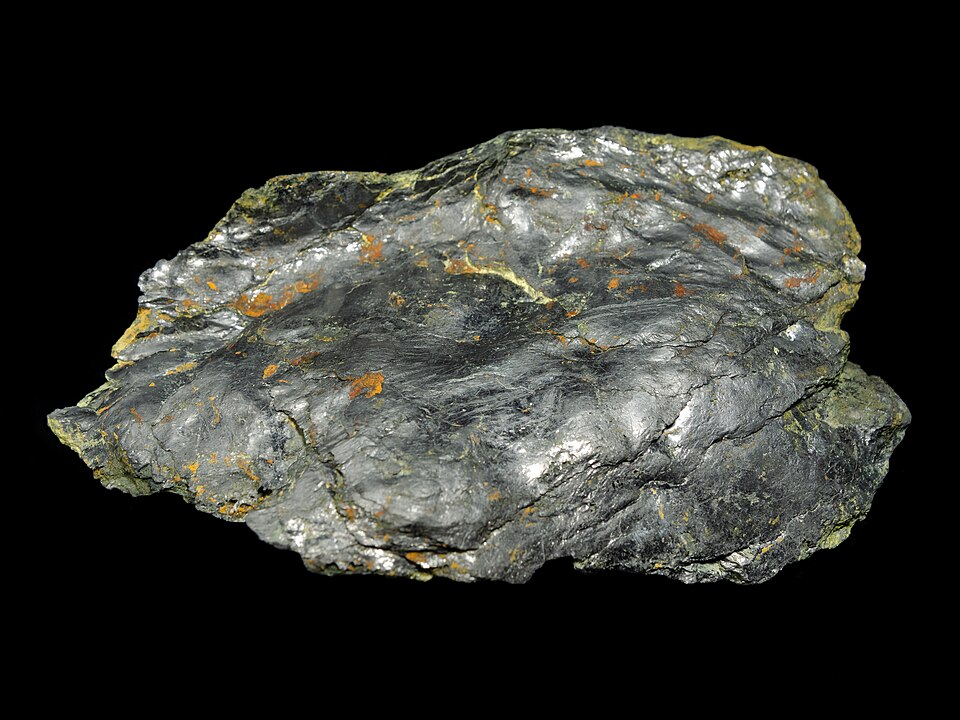
\includegraphics[width=0.36\linewidth]{images/book2/graphite.jpg}

{\small Uma amostra de grafite natural, com seu brilho metálico. Foto:
Zbynek Burival, CC BY-SA 4.0.}
\end{omfigure}

\section{Cristais moleculares}

\begin{definition}[Cristal molecular]\label{def:b1:crystals-ionic-covalent:molecular-crystal}
Um \emph{cristal molecular}\index{cristal molecular} é um \omterm{def:b1:crystals-metals:crystal}{cristal} de
moléculas mantidas unidas por forças intermoleculares --- \omterm{def:b1:intermolecular-forces-solvents:vdw}{interações de
van der Waals} e, quando possível, \omterm{def:b1:intermolecular-forces-solvents:hbond}{ligações de hidrogênio} ---, enquanto
cada molécula conserva suas próprias \omterm{def:b1:lewis-resonance-vsepr:lewis}{ligações covalentes}: o di-iodo, o
gelo-seco \ce{CO2(s)}, o gelo, o açúcar.
\end{definition}

\begin{proposition}[Propriedades dos cristais moleculares]\label{prop:b1:crystals-ionic-covalent:molecular}
Os \omterm{def:b1:crystals-ionic-covalent:molecular-crystal}{cristais moleculares} são moles e fundem ou sublimam a baixas
temperaturas, pois só se rompem forças intermoleculares fracas; eles não
conduzem.
\end{proposition}
\admitted

\begin{example}[O gelo]\label{ex:b1:crystals-ionic-covalent:ice}
No gelo comum, cada molécula de água está ligada por \omterm{def:b1:intermolecular-forces-solvents:hbond}{ligações de
hidrogênio} a outras quatro, nos vértices de um tetraedro: duas por seus
próprios hidrogênios e duas por seus \omterm{def:b1:lewis-resonance-vsepr:lewis}{pares não ligantes}. Essa rede
aberta e hexagonal, imposta pelas direções das \omterm{def:b1:intermolecular-forces-solvents:hbond}{ligações de hidrogênio},
deixa muito espaço vazio: o gelo é menos denso que a água líquida, na
qual a rede está parcialmente rompida e as moléculas se aproximam. A
simetria hexagonal da rede aparece na forma de seis pontas dos \omterm{def:b1:crystals-metals:crystal}{cristais}
de neve.
\end{example}

\begin{omfigure}
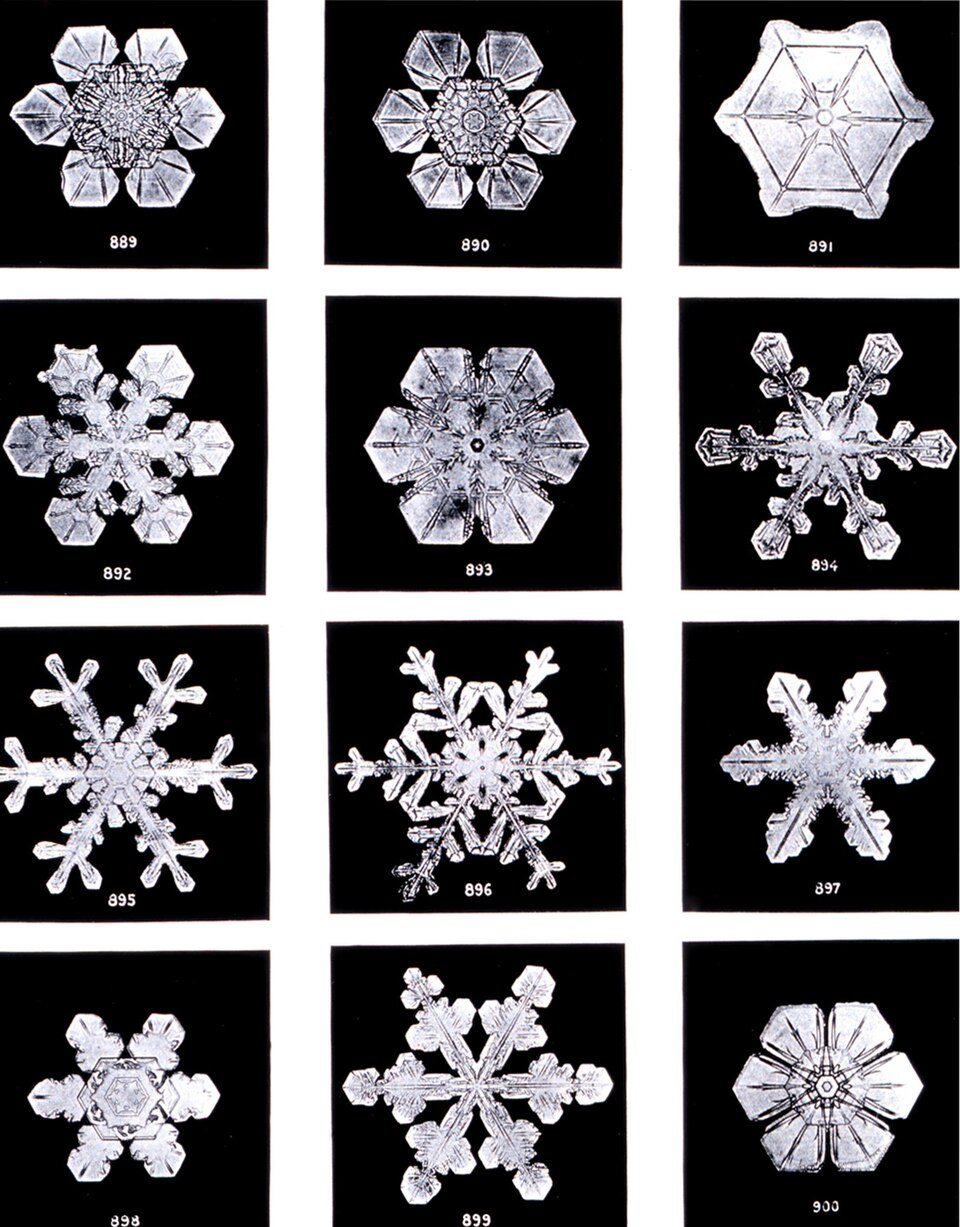
\includegraphics[width=0.38\linewidth]{images/book2/bentley-snowflakes.jpg}

{\small \omterm{def:b1:crystals-metals:crystal}{Cristais} de neve fotografados por Wilson Bentley por volta de
1902: todos têm simetria de ordem seis, marca da rede hexagonal de
\omterm{def:b1:intermolecular-forces-solvents:hbond}{ligações de hidrogênio} do gelo. Domínio público.}
\end{omfigure}

\section{Comparação dos quatro tipos de sólidos}

\begin{center}
\small
\begin{tabular}{lllll}
\hline
sólido & partículas & coesão & propriedades & exemplos \\
\hline
metálico & cátions, elétrons & \omterm{def:b1:crystals-metals:metallic-bond}{ligação metálica} & condutor, dúctil & \ce{Cu}, \ce{Fe}, \ce{Na} \\
iônico & cátions, ânions & eletrostática & duro, quebradiço, isolante & \ce{NaCl}, \ce{CaF2} \\
covalente & átomos & \omterm{def:b1:lewis-resonance-vsepr:lewis}{ligações covalentes} & muito duro, fusão difícil & diamante, \ce{SiO2} \\
molecular & moléculas & van der Waals, lig.\ de H & mole, fusão fácil & \ce{I2}, gelo \\
\hline
\end{tabular}
\end{center}

\begin{remark}[Um contínuo]\label{rem:b1:crystals-ionic-covalent:continuum}
As classes são idealizações. O sulfeto de zinco tem ligações em parte
iônicas, em parte covalentes, e é por isso que sua distância
sulfeto--zinco é menor que a soma dos \omterm{def:b1:periodicity:radius}{raios iônicos}; o grafite é
covalente em suas camadas e molecular entre elas. A diferença de
\omterm{def:b1:periodicity:electronegativity}{eletronegatividade} (\cref{prop:b1:periodicity:en-trend}) é o guia:
quanto maior ela for, mais iônico é o sólido.
\end{remark}

\section{Exercícios}

\begin{exercise}[$\star$]\label{exo:b1:crystals-ionic-covalent:1}
Na célula do sal-gema, conte os cátions e os ânions, dê a coordenação de
cada um e verifique que a fórmula \ce{NaCl} é respeitada.
\end{exercise}

\begin{exercise}[$\star$]\label{exo:b1:crystals-ionic-covalent:2}
O cloreto de césio tem $a = \qty{412.3}{pm}$. Calcule a menor distância
\ce{Cs-Cl} e o número de unidades de fórmula por célula.
\end{exercise}

\begin{exercise}[$\star$]\label{exo:b1:crystals-ionic-covalent:3}
Usando os raios $r(\ce{Na+}) = \qty{102}{pm}$ e $r(\ce{Cl-}) =
\qty{181}{pm}$, calcule a \omterm{def:b1:crystals-ionic-covalent:radius-ratio}{razão de raios} de \ce{NaCl} e preveja a
coordenação do cátion.
\end{exercise}

\begin{exercise}[$\star$]\label{exo:b1:crystals-ionic-covalent:4}
Classifique como metálico, iônico, covalente ou molecular: cobre,
cloreto de sódio, diamante, di-iodo, quartzo \ce{SiO2}, gelo, fluoreto
de cálcio.
\end{exercise}

\begin{exercise}[$\star\star$]\label{exo:b1:crystals-ionic-covalent:5}
Demonstre que a estrutura do sal-gema exige $r_+/r_- \ge \sqrt2 - 1$.
\end{exercise}

\begin{exercise}[$\star\star$]\label{exo:b1:crystals-ionic-covalent:6}
Calcule a massa específica do cloreto de sódio a partir de
$a = \qty{564.1}{pm}$ ($M(\ce{NaCl}) = \qty{58.44}{g/mol}$) e compare
com \qty{2.17}{g/cm^3}.
\end{exercise}

\begin{exercise}[$\star\star$]\label{exo:b1:crystals-ionic-covalent:7}
Calcule a massa específica do cloreto de césio ($M = \qty{168.36}{g/mol}$,
$a = \qty{412.3}{pm}$) e compare com o valor medido, \qty{3.99}{g/cm^3}.
% ledger: rho:CsCl
\end{exercise}

\begin{exercise}[$\star\star$]\label{exo:b1:crystals-ionic-covalent:8}
Para a blenda ($a = \qty{540.9}{pm}$, $M = \qty{97.44}{g/mol}$), calcule
a distância \ce{Zn-S} e a massa específica, e compare com o valor medido,
\qty{4.04}{g/cm^3}.
% ledger: rho:ZnS
\end{exercise}

\begin{exercise}[$\star\star$]\label{exo:b1:crystals-ionic-covalent:9}
O grafite tem uma célula hexagonal com $a = \qty{245.6}{pm}$ e
$c = \qty{669.6}{pm}$, que contém 4 átomos. Calcule a distância \ce{C-C}
em uma camada ($a/\sqrt3$), a distância entre camadas ($c/2$) e a massa
específica. Por que o grafite é menos denso que o diamante?
\end{exercise}

\begin{exercise}[$\star\star\star$]\label{exo:b1:crystals-ionic-covalent:10}
Demonstre que a \omterm{def:b1:crystals-metals:compactness}{compacidade} do diamante é $\pi\sqrt3/16$, e explique por
que o material mais duro é um dos menos compactos.
\end{exercise}

\begin{exercise}[$\star\star\star$]\label{exo:b1:crystals-ionic-covalent:11}
O silício tem a estrutura do diamante com $a = \qty{543.1}{pm}$. Calcule
o comprimento da ligação \ce{Si-Si}, o \omterm{def:b1:periodicity:radius}{raio covalente} do silício e a
massa específica ($M = \qty{28.09}{g/mol}$); compare com \qty{2.33}{g/cm^3}.
\end{exercise}

\begin{exercise}[$\star\star\star$]\label{exo:b1:crystals-ionic-covalent:12}
O cloreto de rubídio tem $r(\ce{Rb+}) = \qty{152}{pm}$ (seis vizinhos) e
$r(\ce{Cl-}) = \qty{181}{pm}$. Que estrutura a regra da \omterm{def:b1:crystals-ionic-covalent:radius-ratio}{razão de raios}
prevê? Em condições ordinárias, ele é do \omterm{def:b1:crystals-ionic-covalent:structure-type}{tipo sal-gema} com
$a = \qty{658.1}{pm}$: verifique a distância \ce{Rb-Cl} e sugira por que
a regra falha aqui.
% ledger: rion:Rb+VI, rion:Cl-VI, lat:RbCl
\end{exercise}

\section{Problema: A fluorita, o mineral e a lente}

\begin{problem}[{Problema de fim de semana --- a célula da fluorita, sua
\omterm{def:b1:crystals-ionic-covalent:radius-ratio}{razão de raios}, dois parentes (\ce{Li2O} e o diamante) e a massa
específica da fluorita calculada a partir de sua célula}]
\label{pb:b1:crystals-ionic-covalent:1}
A fluorita, \ce{CaF2}, é um mineral; crescida em grandes \omterm{def:b1:crystals-metals:crystal}{cristais}
límpidos, ela fornece lentes que transmitem a luz ultravioleta. Sua
célula é cúbica, $a =
\qty{546.3}{pm}$; \ce{Ca^{2+}} em uma \omterm{def:b1:crystals-metals:lattice}{rede} CFC, \ce{F-} nos \omterm{def:b1:crystals-metals:site}{sítios
tetraédricos}. Raios: $r(\ce{Ca^{2+}}) = \qty{112}{pm}$ (oito
vizinhos), $r(\ce{F-}) = \qty{131}{pm}$ (quatro vizinhos). Massas molares
(g/mol): \ce{Ca} 40.08, \ce{F} 19.00, \ce{Li} 6.94, \ce{O} 16.00, \ce{C}
12.01, \ce{Si} 28.09; $N_A = \qty{6.022e23}{mol^{-1}}$.
% ledger: lat:CaF2, rion:Ca2+VIII, rion:F-IV, aw:Ca, aw:F, aw:Li, aw:O,
% aw:C, aw:Si, const:NA

\medskip
\noindent\textbf{Parte I --- A célula.}
\begin{enumerate}
  \item Dê as posições dos íons \ce{Ca^{2+}} na célula e conte-os.
  \item Quantos \omterm{def:b1:crystals-metals:site}{sítios tetraédricos} a célula contém? Deduza o número de
        íons \ce{F-} e verifique a fórmula.
  \item Qual é a coordenação de \ce{F-}? E a de \ce{Ca^{2+}}?
  \item Calcule a menor distância \ce{Ca-F}.
  \item Compare-a com a soma dos \omterm{def:b1:periodicity:radius}{raios iônicos}.
  \item Calcule a menor distância \ce{F-F} e diga se os ânions se tocam.
\end{enumerate}

\medskip
\noindent\textbf{Parte II --- A \omterm{def:b1:crystals-ionic-covalent:radius-ratio}{razão de raios}.}
\begin{enumerate}[resume]
  \item Calcule $x = r_+/r_-$.
  \item Que coordenação do cátion a regra da \omterm{def:b1:crystals-ionic-covalent:radius-ratio}{razão de raios} permite?
  \item Por que \ce{CaF2} não pode adotar a estrutura do cloreto de césio,
        embora seu cátion tenha coordenação 8?
  \item Descreva a fluorita como um arranjo cúbico simples de \ce{F-} com
        \ce{Ca^{2+}} nos centros da metade dos cubinhos.
  \item Calcule a \omterm{def:b1:crystals-metals:compactness}{compacidade} da fluorita.
\end{enumerate}

\medskip
\noindent\textbf{Parte III --- Dois parentes.}
O óxido de lítio, \ce{Li2O}, é antifluorita com $a = \qty{461.9}{pm}$;
$r(\ce{Li+}) = \qty{59}{pm}$ (quatro vizinhos), $r(\ce{O^{2-}}) =
\qty{142}{pm}$ (oito vizinhos). Diamante: $a = \qty{356.7}{pm}$.
% ledger: lat:Li2O, rion:Li+IV, rion:O2-VIII, rho:Li2O, lat:C-diamond
\begin{enumerate}[resume]
  \item Onde ficam os íons \ce{O^{2-}} e \ce{Li+} na célula da
        antifluorita?
  \item Calcule a distância \ce{Li-O} e compare com a soma dos raios.
  \item Calcule a massa específica de \ce{Li2O} e compare com o valor
        medido, \qty{2.01}{g/cm^3}.
  \item Que estrutura iônica tem o mesmo arranjo de posições que o
        diamante?
  \item Calcule o comprimento da ligação \ce{C-C} e a massa específica
        do diamante.
  \item Por que o diamante é tão menos compacto que a fluorita, embora
        seus átomos ocupem o mesmo tipo de posições?
\end{enumerate}

\medskip
\noindent\textbf{Parte IV --- A massa específica da fluorita.}
\begin{enumerate}[resume]
  \item Calcule a massa molar de \ce{CaF2}.
  \item Calcule a massa de uma célula.
  \item Calcule o volume de uma célula, em \unit{cm^3}.
  \item Que efeito teria sobre a massa específica uma lacuna em um sítio
        \ce{F-} a cada cem células?
  \item Calcule a massa específica da fluorita a partir de sua célula e
        compare-a com o valor medido, \qty{3.18}{g/cm^3}.
\end{enumerate}
% ledger: rho:CaF2
\end{problem}
